\chapter{Darts}

This project represents the popular darts game. The player shoots short arrows at a circular target. The closer it is to the center of the target, the more points it earns. The goal of the player is to collect the maximum number of points for the three shots available. If the collected points are more than 13 - win the game, otherwise lose the game.

\begin{figure}[H]
   \centering
   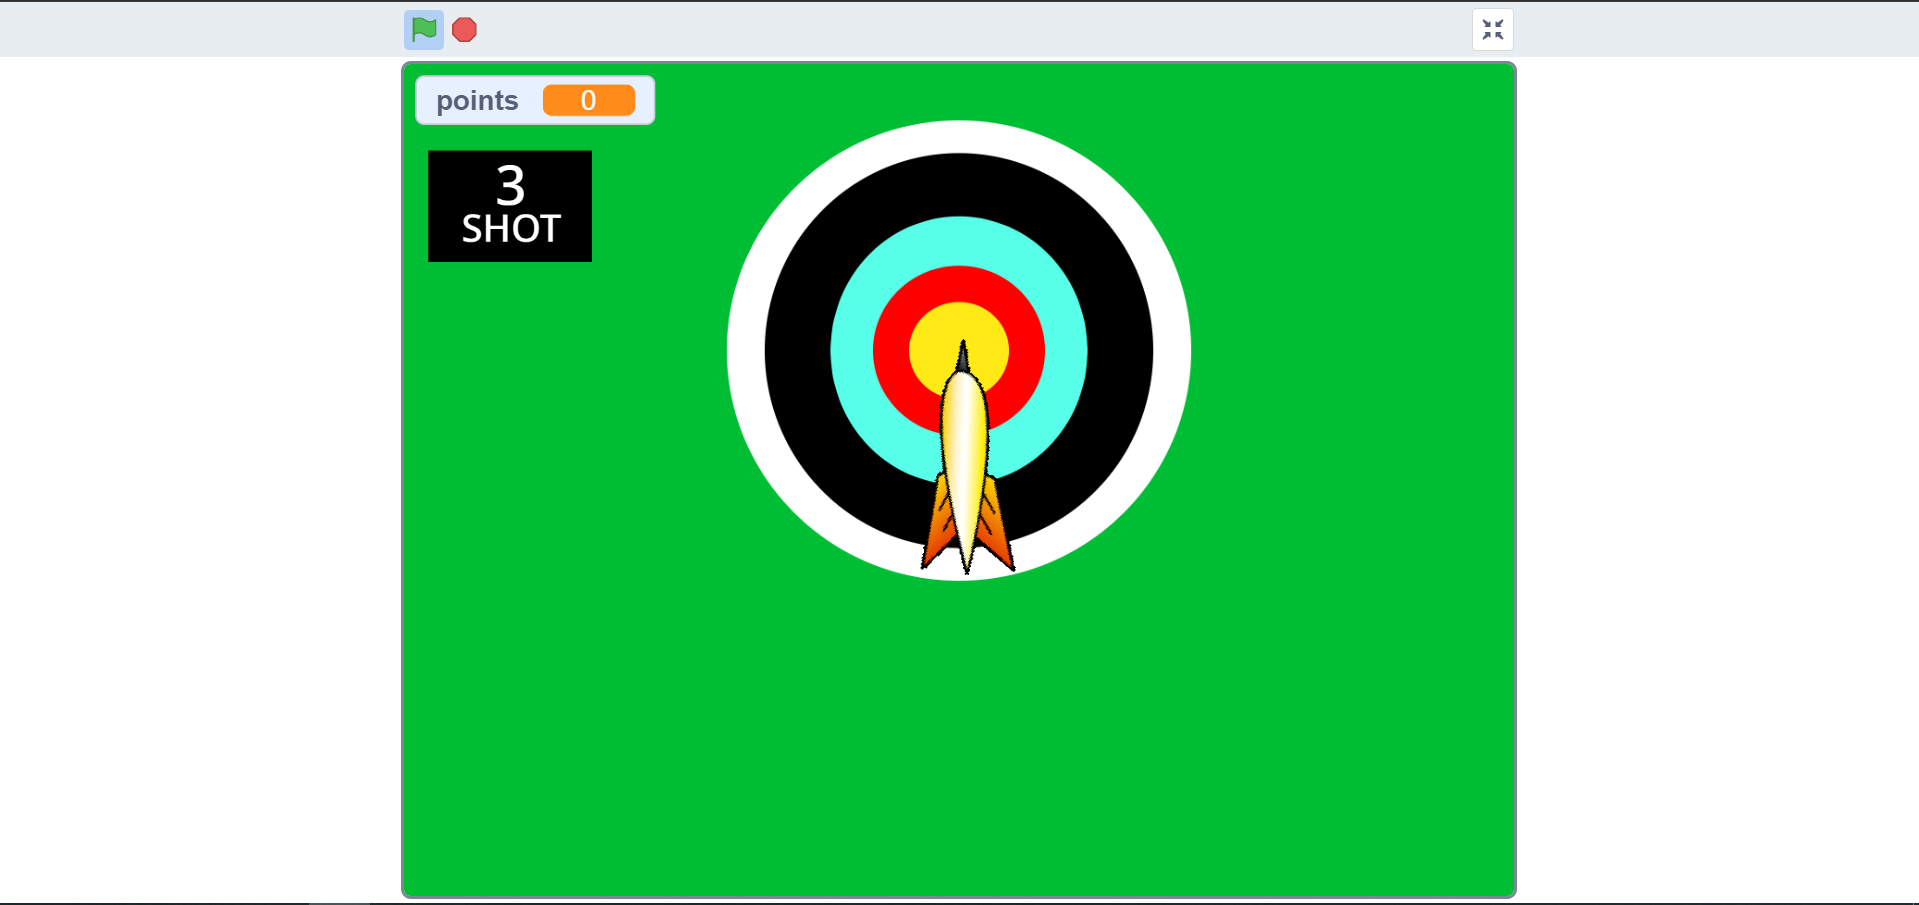
\includegraphics[width=1.0\linewidth,height=0.5\linewidth]{fig150001.png}
   \caption{Darts}
\label{fig150001}
\end{figure}

\section{Creating the Design}
Before you start programming the game, you must first create the design. First, add the two main characters of the game - the target (Fig. \ref{fig150002}) and the arrow (Fig. \ref{fig150003}). Use the tools in Scratch to draw the required characters.

\begin{figure}[H]
   \centering
   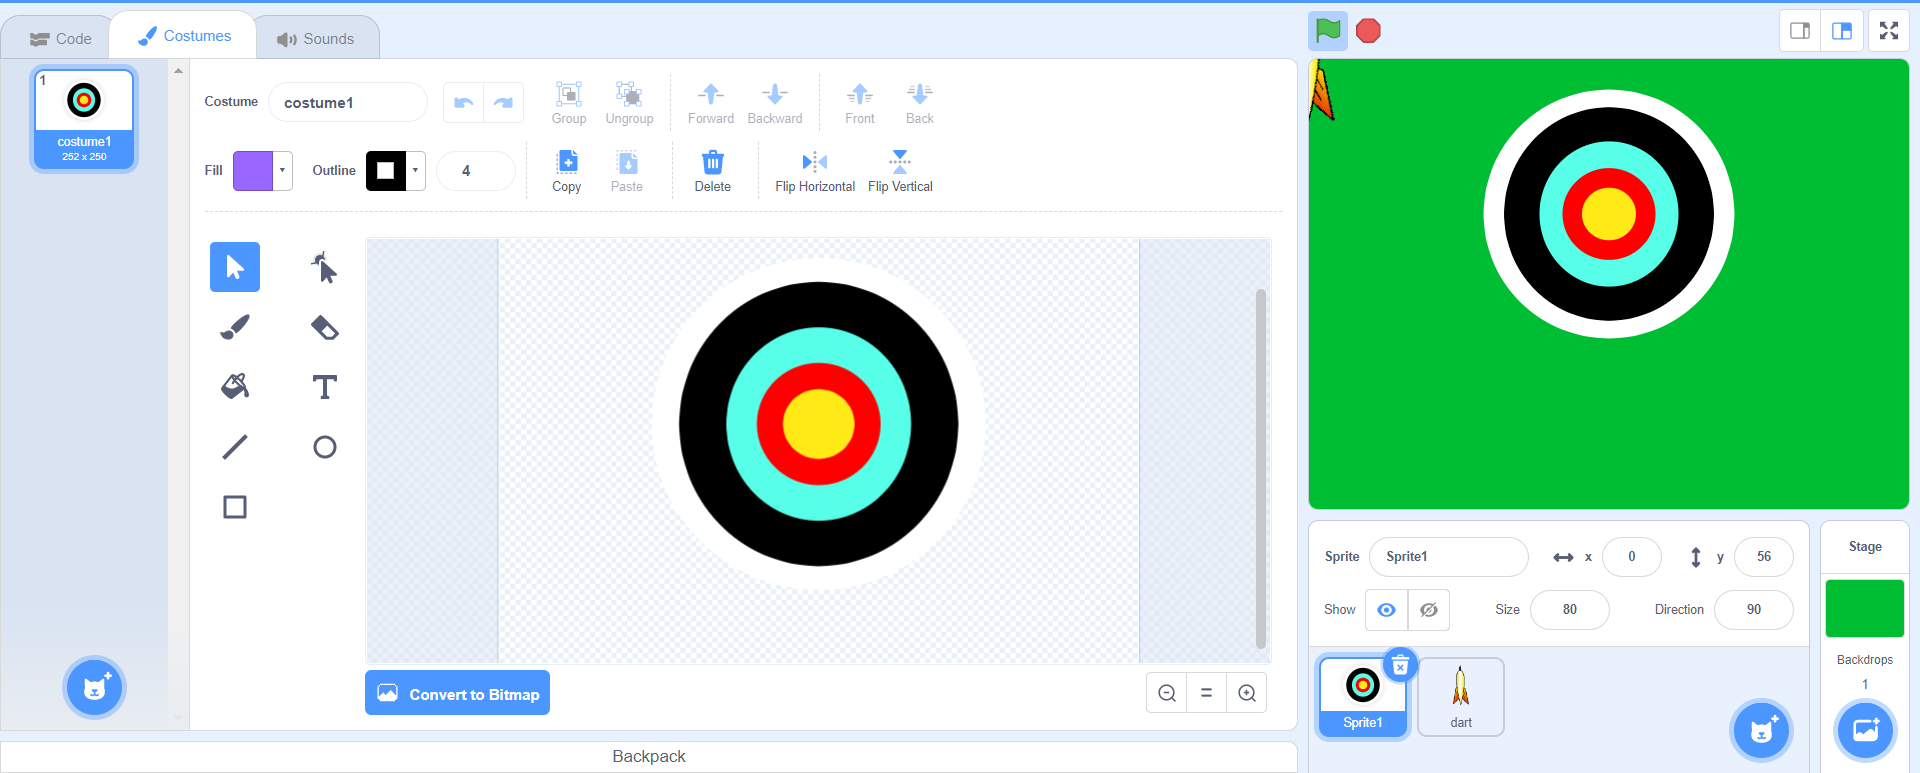
\includegraphics[width=1.0\linewidth,height=0.5\linewidth]{fig150002.png}
   \caption{Target}
\label{fig150002}
\end{figure}

\begin{figure}[H]
   \centering
   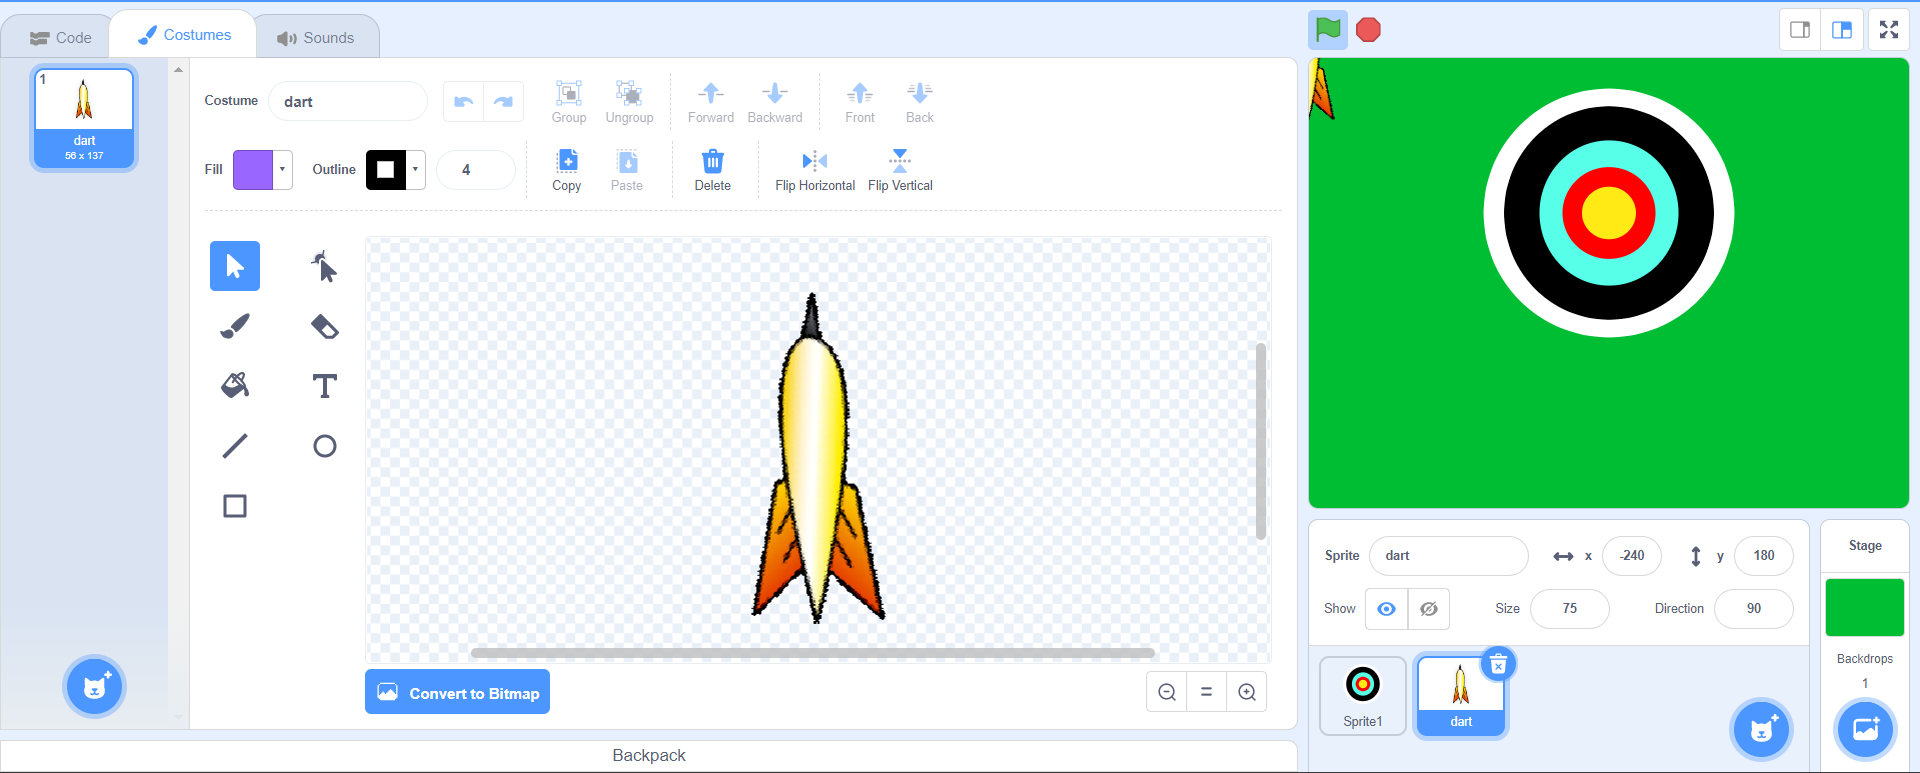
\includegraphics[width=1.0\linewidth,height=0.5\linewidth]{fig150003.png}
   \caption{Arrow}
\label{fig150003}
\end{figure}

Add a new character that you can also draw using the Scratch tools. This character will be responsible for showing how many shots the player has left. To show how many shots are left, add costumes to that character. For example, on the first suit you can write that there are 3 shots left, and on the second - 2 shots.

\begin{figure}[H]
   \centering
   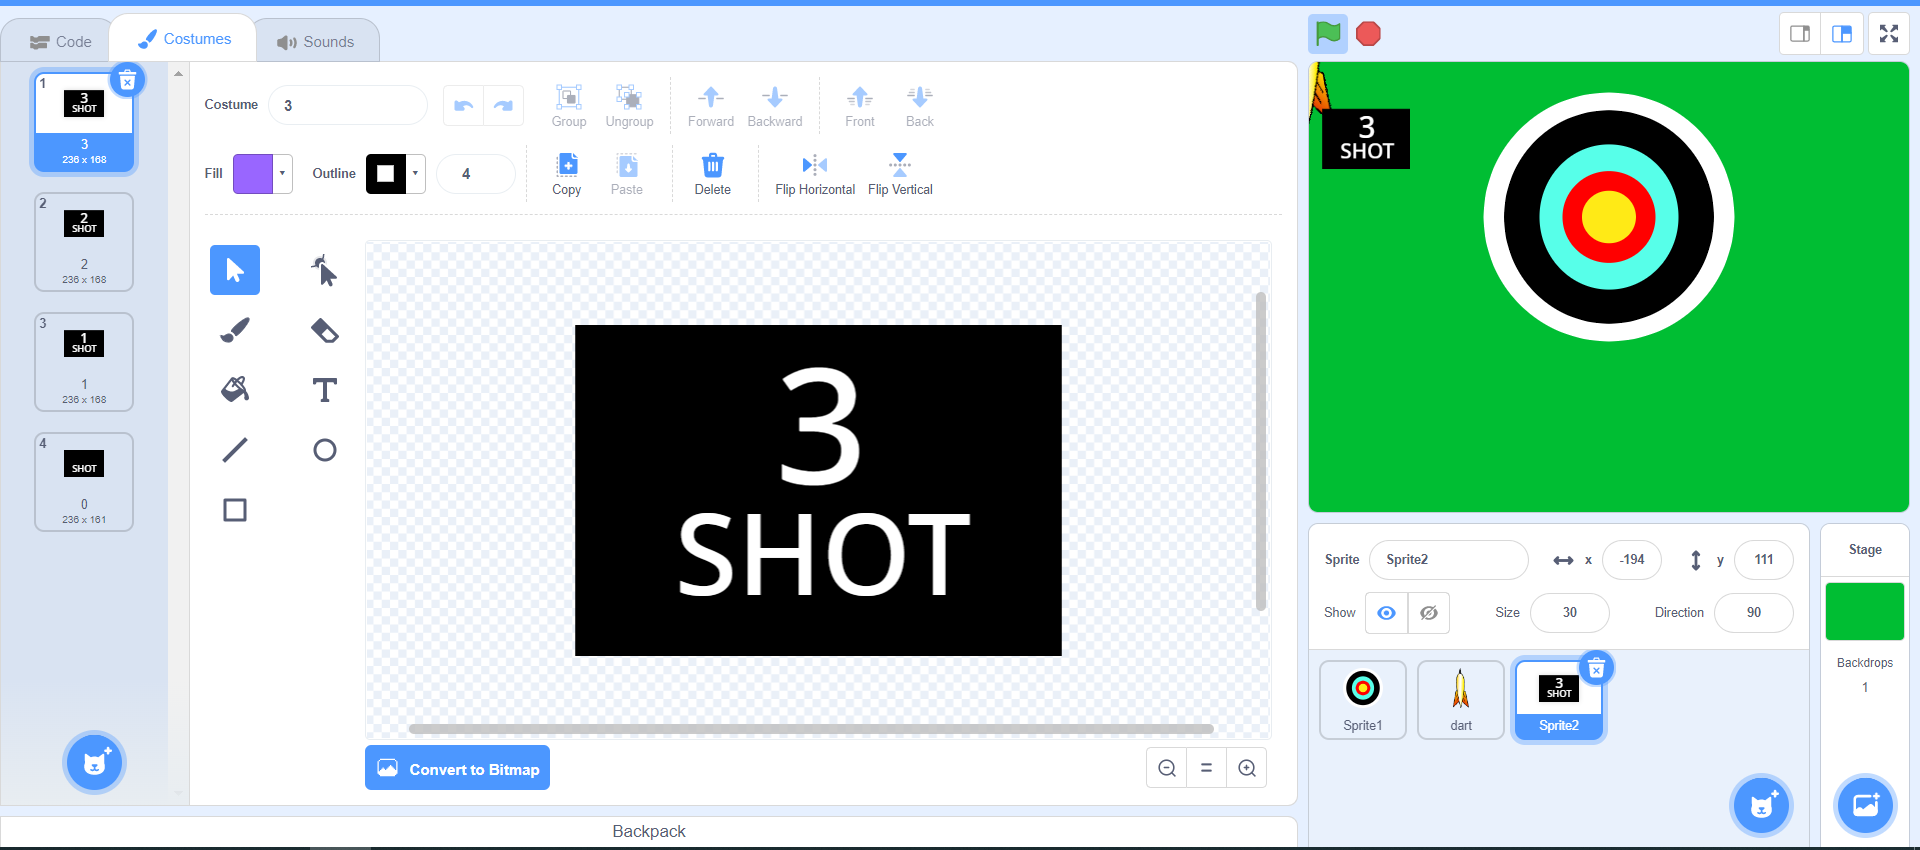
\includegraphics[width=1.0\linewidth,height=0.5\linewidth]{fig150004.png}
   \caption{Number of Shots}
\label{fig150004}
\end{figure}

The next character to add is the one that shows how many points the player has earned. Again, add costumes to the character with the corresponding number of points he can earn. In this case, these are from 0 to 5.

\begin{figure}[H]
   \centering
   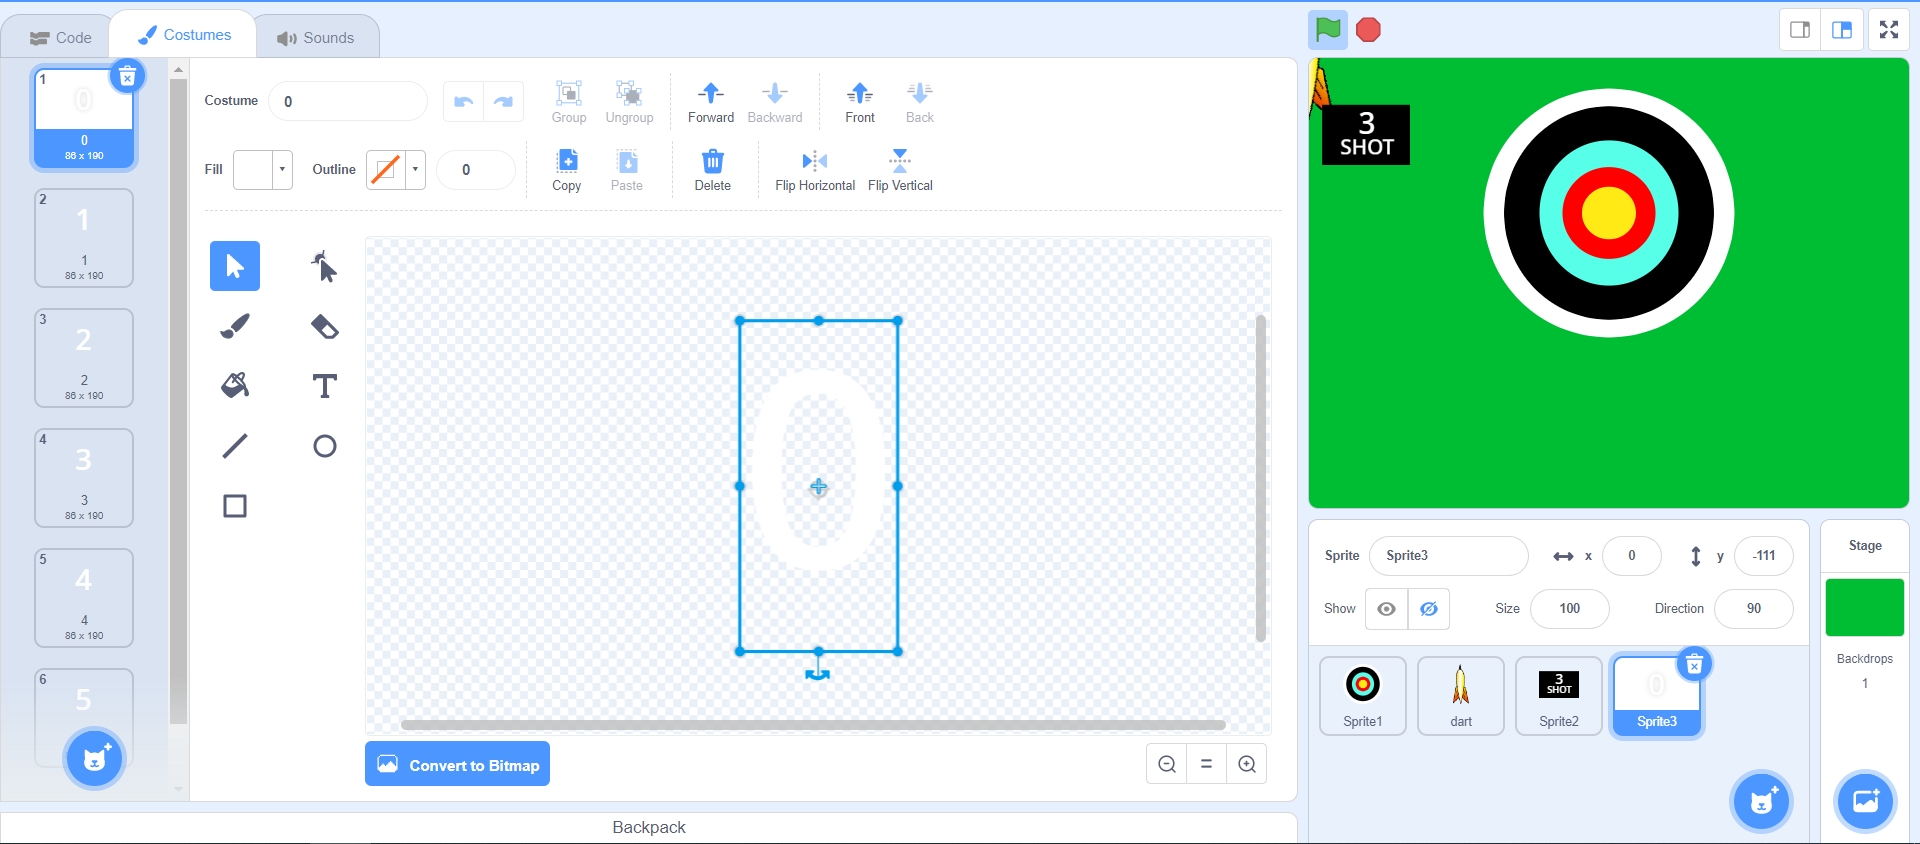
\includegraphics[width=1.0\linewidth,height=0.5\linewidth]{fig150005.png}
   \caption{Number of points}
\label{fig150005}
\end{figure}

The last Scratch character is the inscription whether the player wins or loses. Like the previous two characters, add two suits with different inscriptions - one for winning and the other for losing.

\begin{figure}[H]
   \centering
   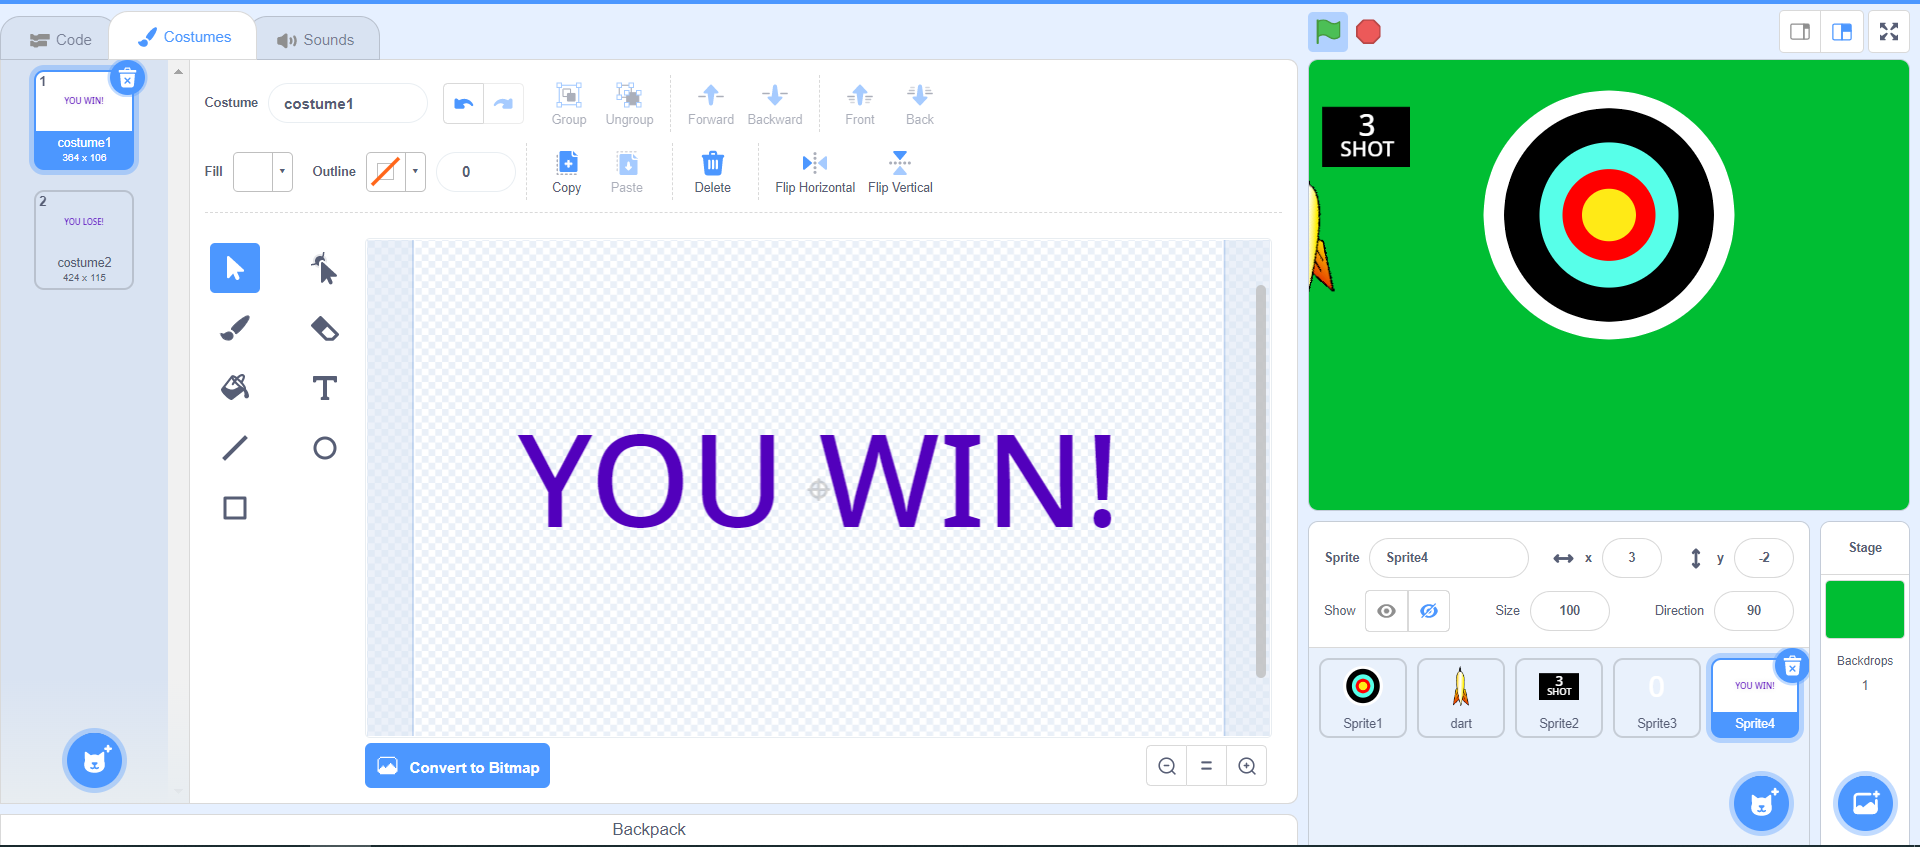
\includegraphics[width=1.0\linewidth,height=0.5\linewidth]{fig150006.png}
   \caption{End of Game Caption}
\label{fig150006}
\end{figure}

\section{Programming the target and boom}
Before we move on to programming the respective characters, add a new variable points to the game. This variable will contain the score that the character will accumulate during the game. From the Variables section, select Make a Variable and name the variable.

\begin{figure}[H]
   \centering
   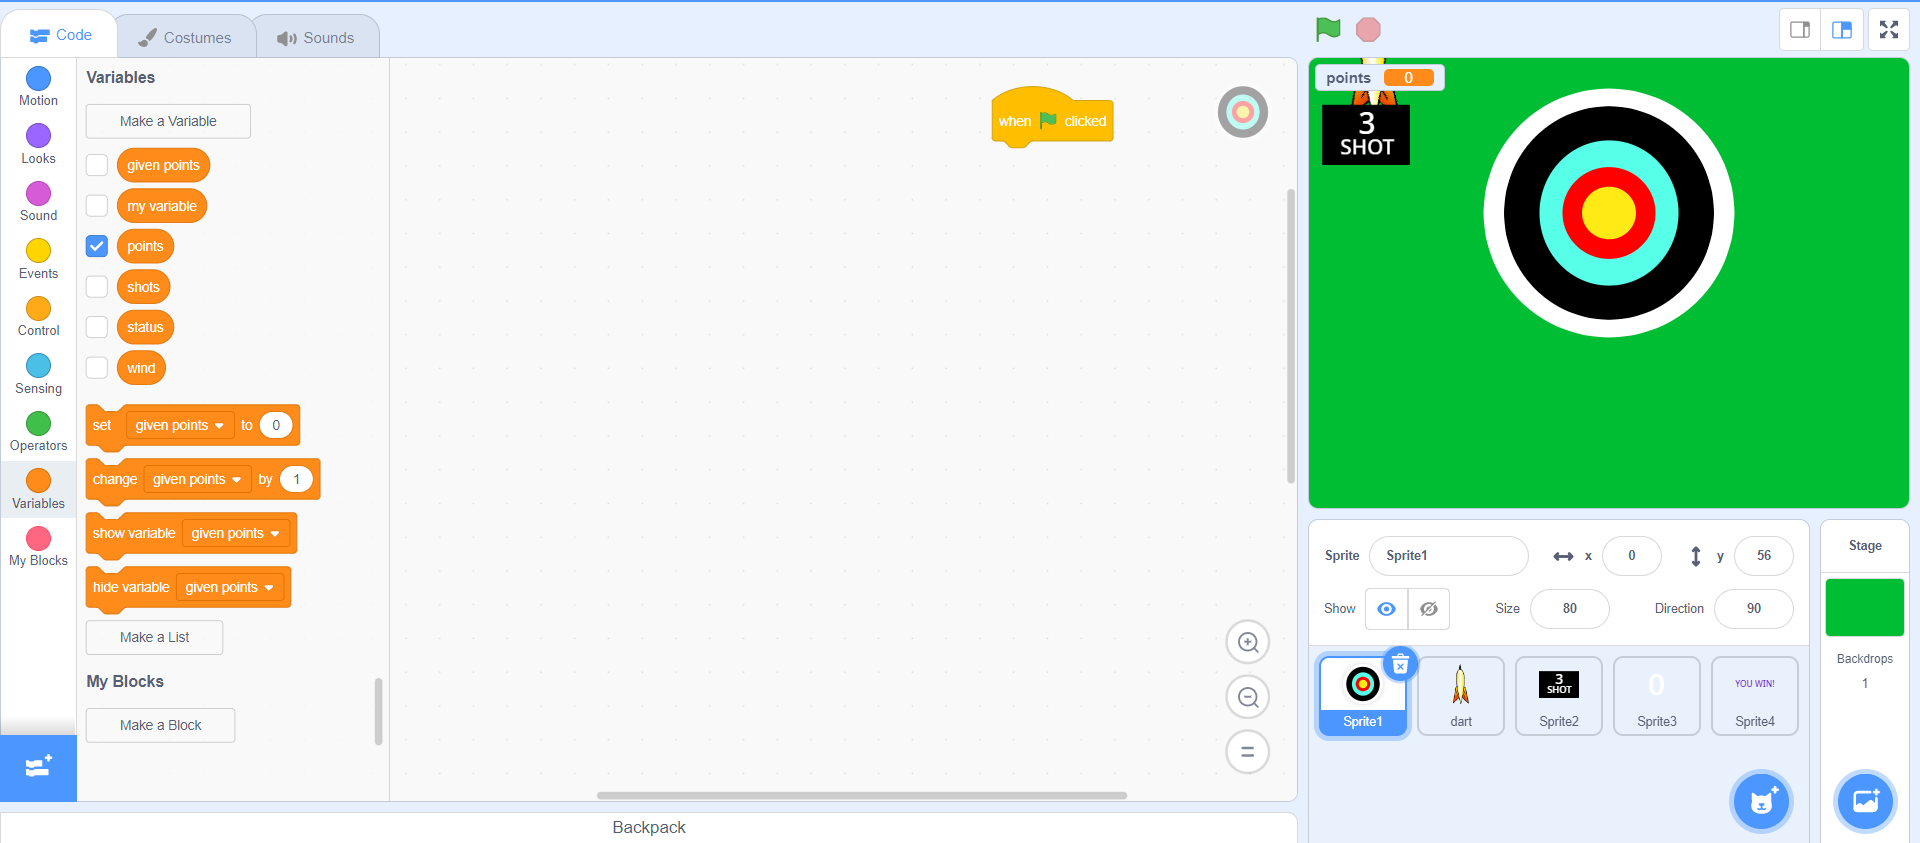
\includegraphics[width=1.0\linewidth,height=0.5\linewidth]{fig150007.png}
   \caption{Creating in-game variable}
\label{fig150007}
\end{figure}

Let's move on to programming the target. The only instructions you need to add to this character are that it stays in the same position throughout the game. Don't forget to also set an initial value to the variable you created. At the beginning of each game, the player must have 0 points.

\begin{figure}[H]
   \centering
   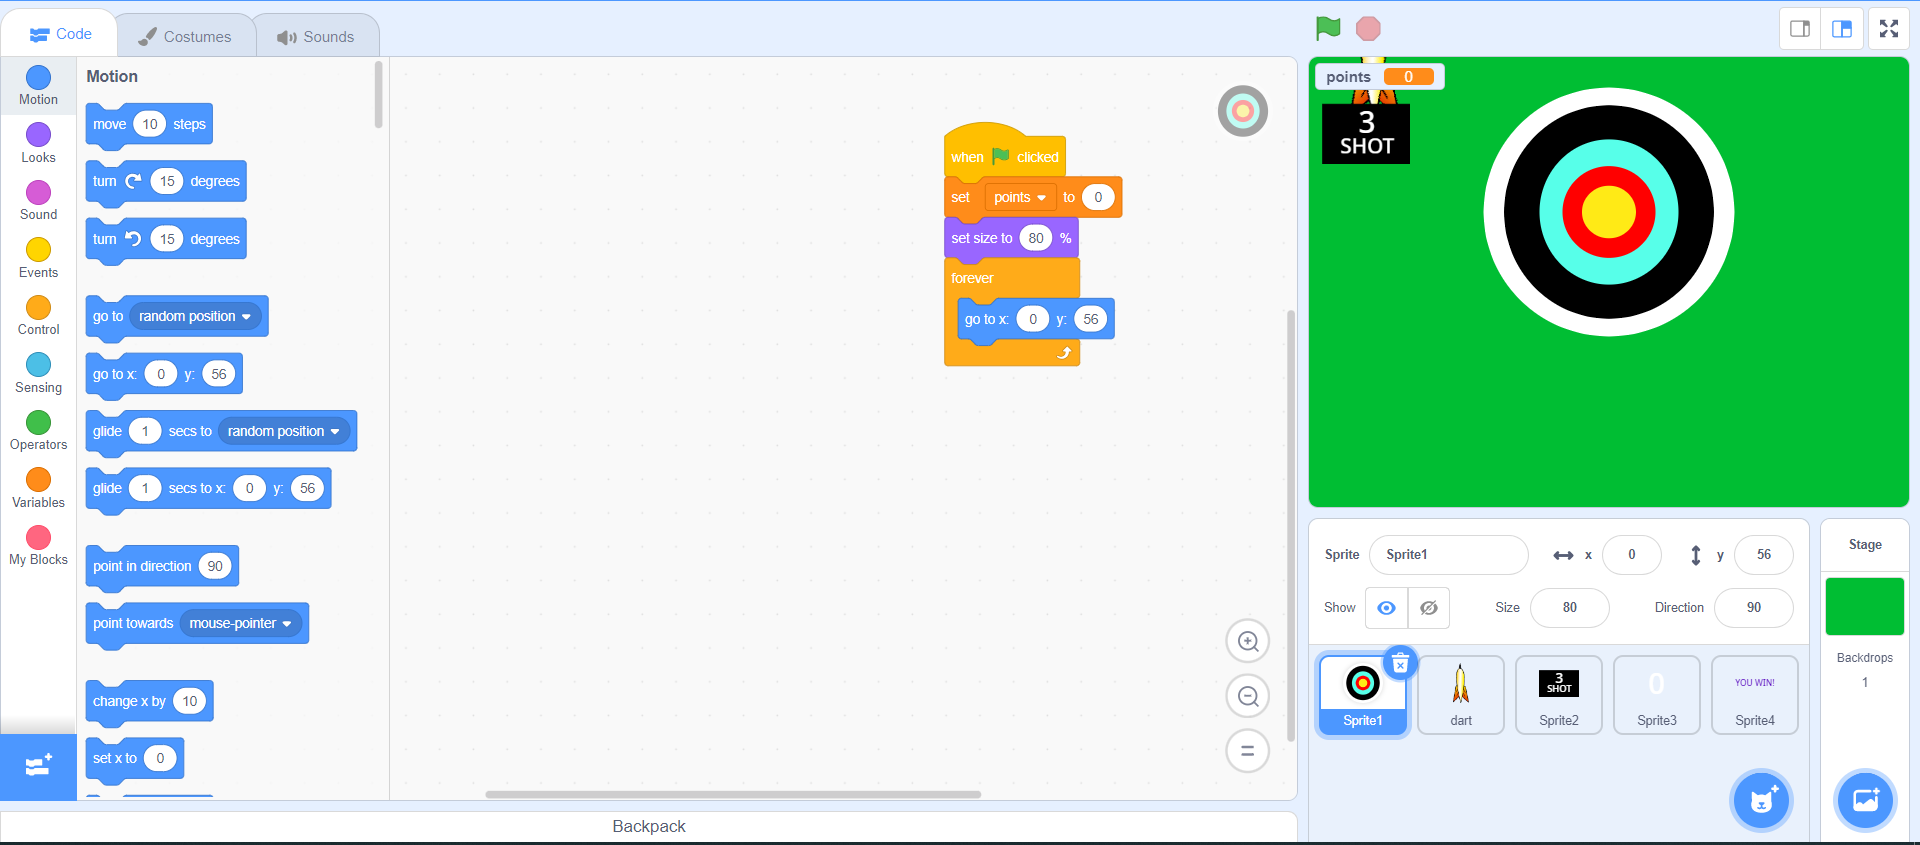
\includegraphics[width=1.0\linewidth,height=0.5\linewidth]{fig150008.png}
   \caption{Target instructions}
\label{fig150008}
\end{figure}

You should also add instructions for the arrow. If the arrow is too big, you can resize it. Create a new variable to hold what the status of the arrow is. There are two statuses - shoot or throw. At the start of the game, the status of the arrow will be shoot.

\begin{figure}[H]
   \centering
   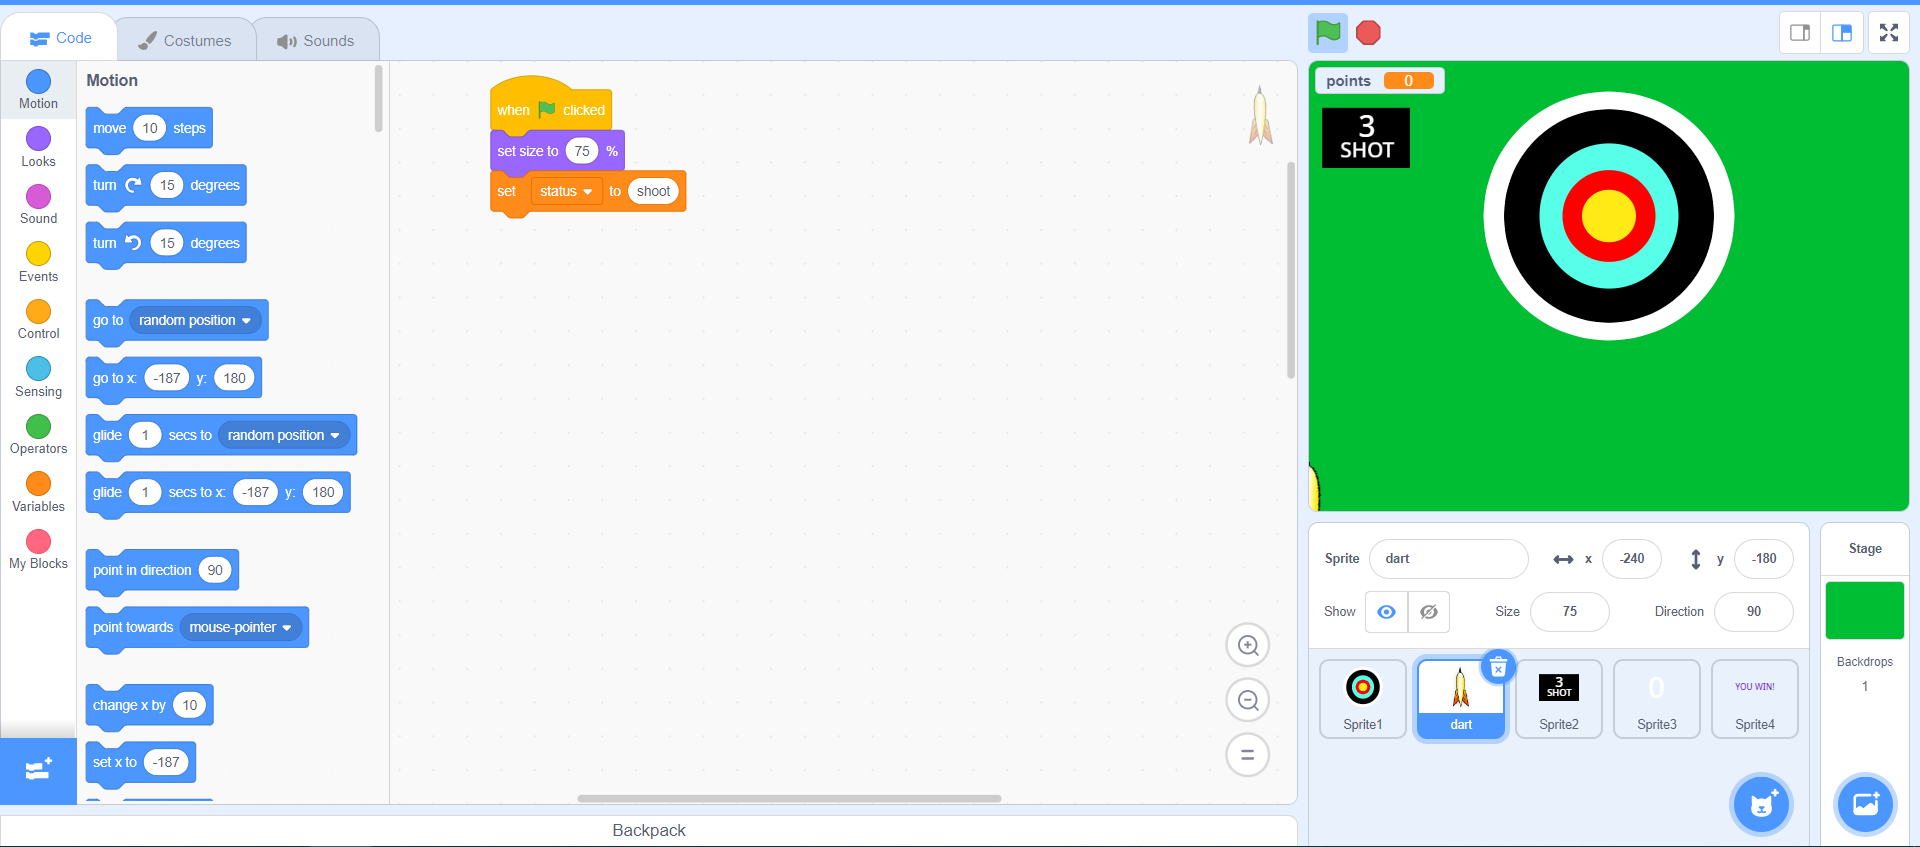
\includegraphics[width=1.0\linewidth,height=0.5\linewidth]{fig150009.png}
   \caption{Set Arrow Status}
\label{fig150009}
\end{figure}

Add the following check - if the arrow's status is shoot, then the arrow must follow the player's mouse. Also add a new event which is when this sprite clicked. When the player clicks the arrow, you need to change the value of the status variable to throw. Also, the character must send a message to the other characters that the player has clicked the mouse, which means he is shooting.

\begin{figure}[H]
   \centering
   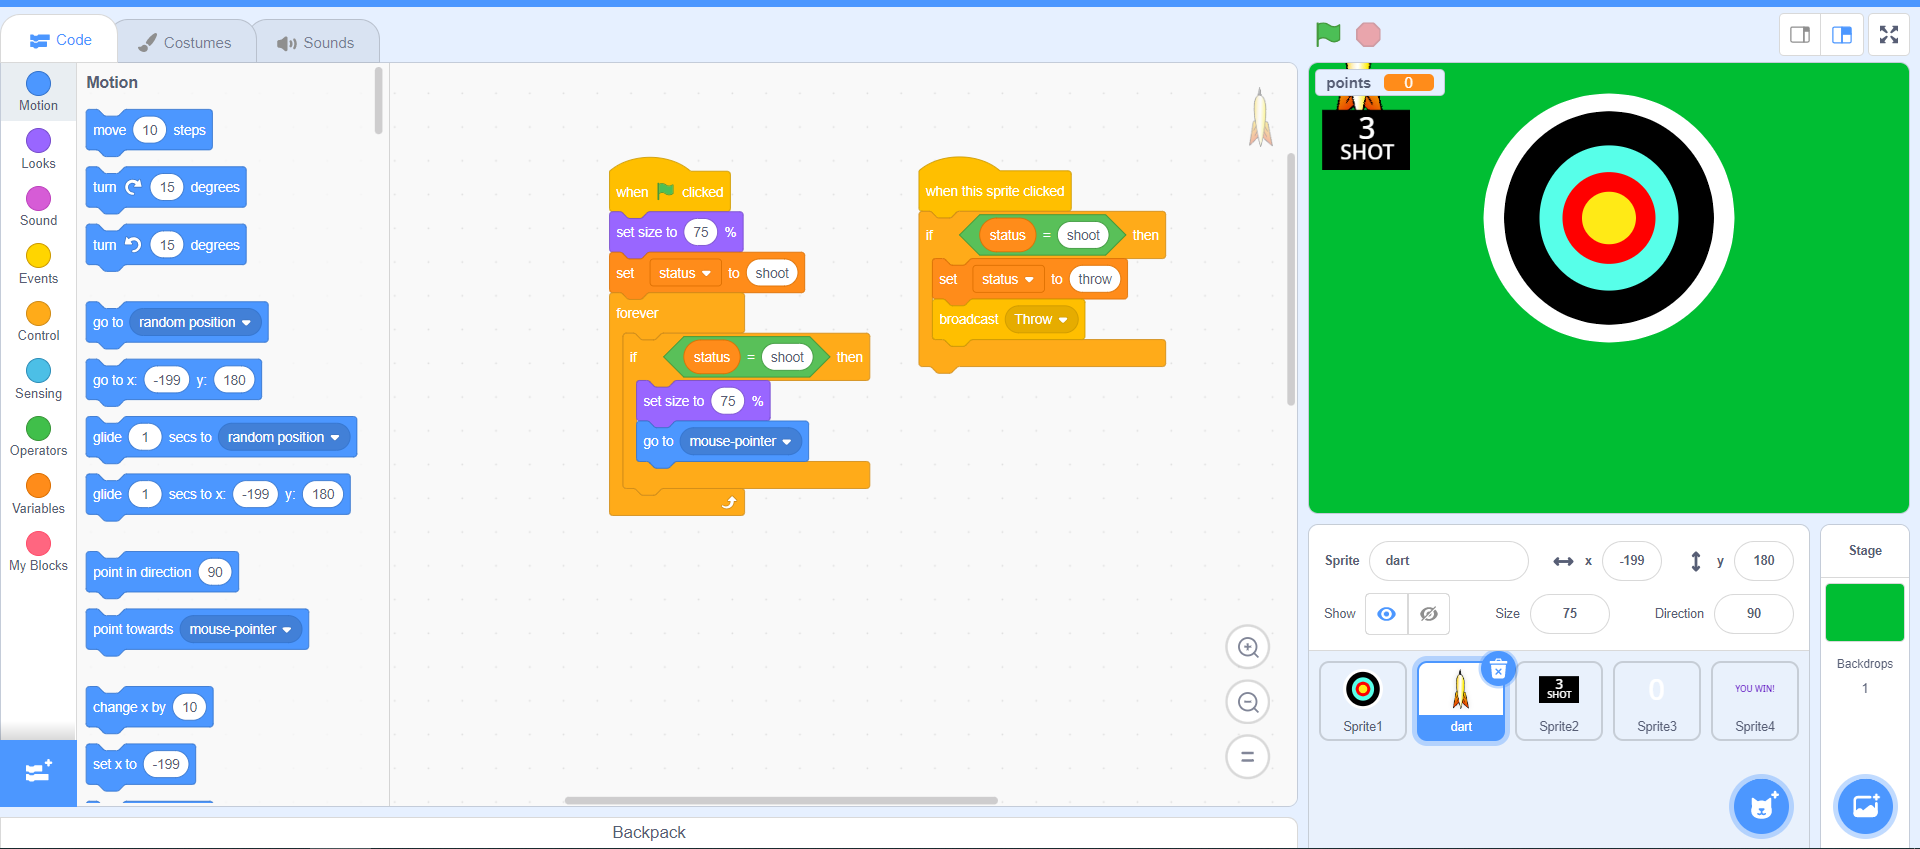
\includegraphics[width=1.0\linewidth,height=0.5\linewidth]{fig150010.png}
   \caption{Send shooting message}
\label{fig150010}
\end{figure}

After the player has fired the arrow you need to program it to change its direction so that you can imitate a shot. Also resize it to make it smaller, as if it is moving away from the player. You know that when the player clicks on the arrow, it sends a message. Use this message to change the direction and size of the arrow after firing.

\begin{figure}[H]
   \centering
   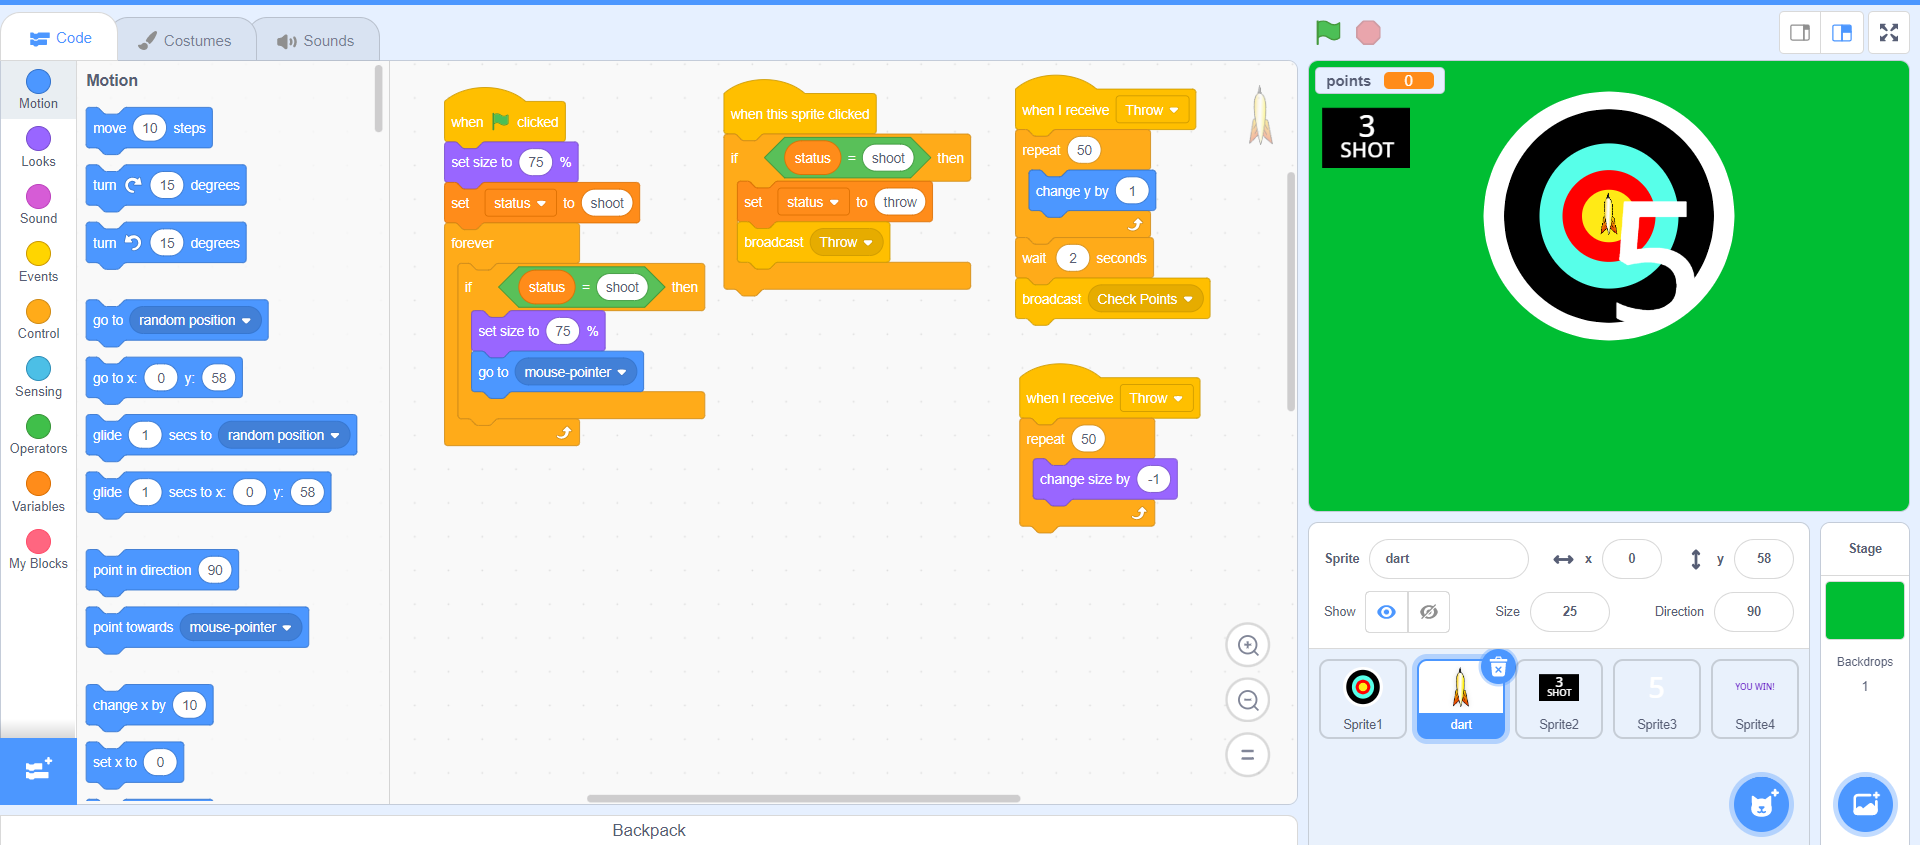
\includegraphics[width=1.0\linewidth,height=0.5\linewidth]{fig150011.png}
   \caption{Change arrow direction and size after shot}
\label{fig150011}
\end{figure}

When the player fires the arrow, it starts moving away and sends a Check Points message, which should check how many points the player has earned. To determine the number of points earned, it is necessary to check what color the arrow touched. In order for the game to be fairest, the check that will be made is the black color (this is the tip of the arrow) to which color it has touched. Add a new variable to hold the currently earned points. The last instruction to add is for the arrow to send a message that it gives points to the player.

\begin{figure}[H]
   \centering
   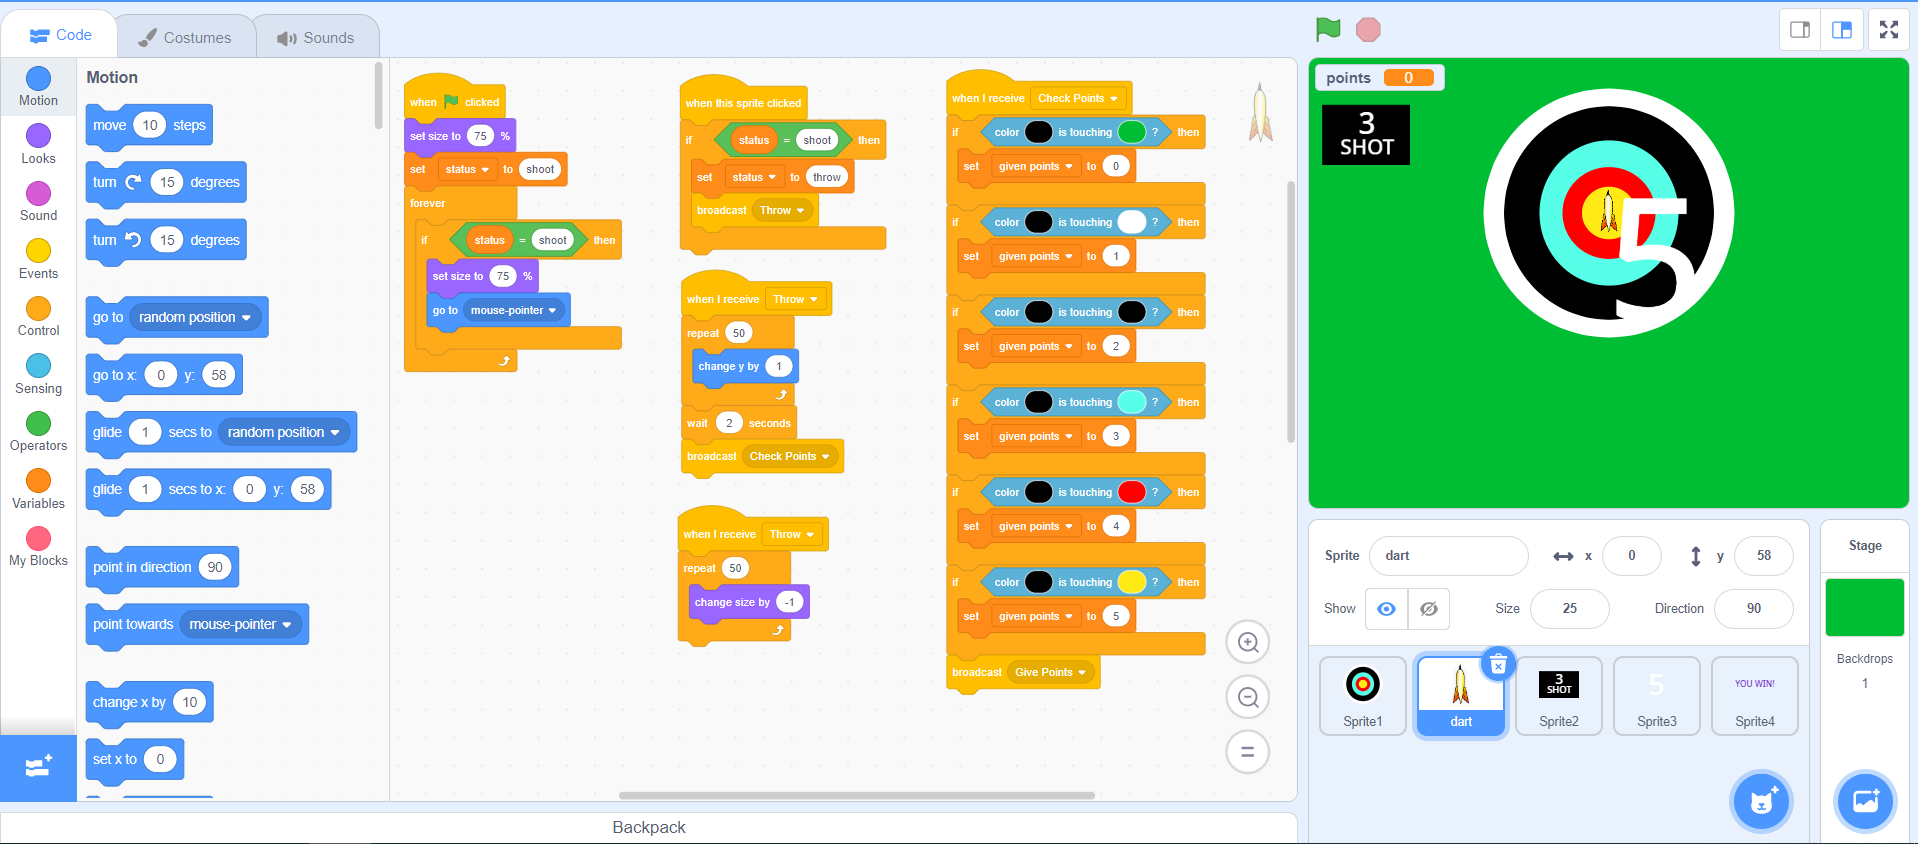
\includegraphics[width=1.0\linewidth,height=0.5\linewidth]{fig150012.png}
   \caption{Check Points Earned}
\label{fig150012}
\end{figure}

To make the game even more interesting, you can add a variable to be a randomly assigned number. This variable will deflect the arrow to the side depending on what random number has landed.

\begin{figure}[H]
   \centering
   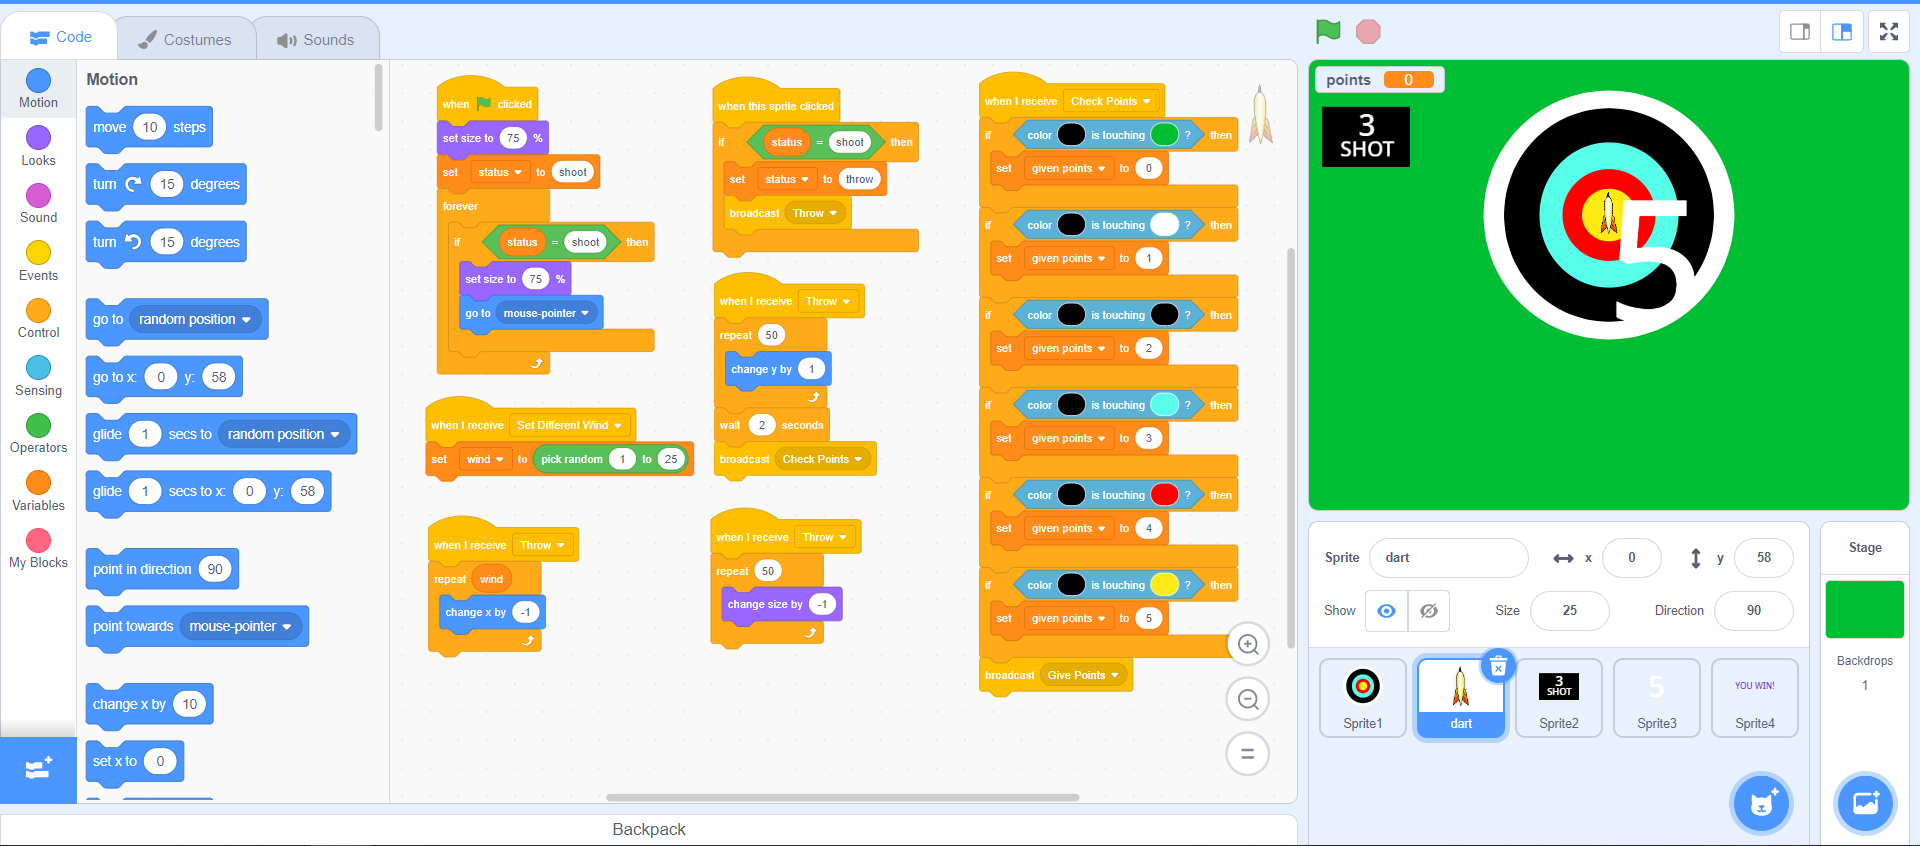
\includegraphics[width=1.0\linewidth,height=0.5\linewidth]{fig150013.png}
   \caption{Arrow deflection to the side}
\label{fig150013}
\end{figure}

\section{Programming the character that counts the number of shots}

In this step, you will add instructions that will show the player how many more shots he is allowed to make. To do this, select the character you added for the number of shots. Place this character in a position of your choice. Create a new variable that will contain the number of shots fired. Then make the necessary checks - if the number of shots is 3, then one should switch to a suit that shows three shots, if the number of shots is two - then one should switch to the suit with two shots, and so on. At the last check - if the number of shots is 0, then a message should be sent that the game is over.

\begin{figure}[H]
   \centering
   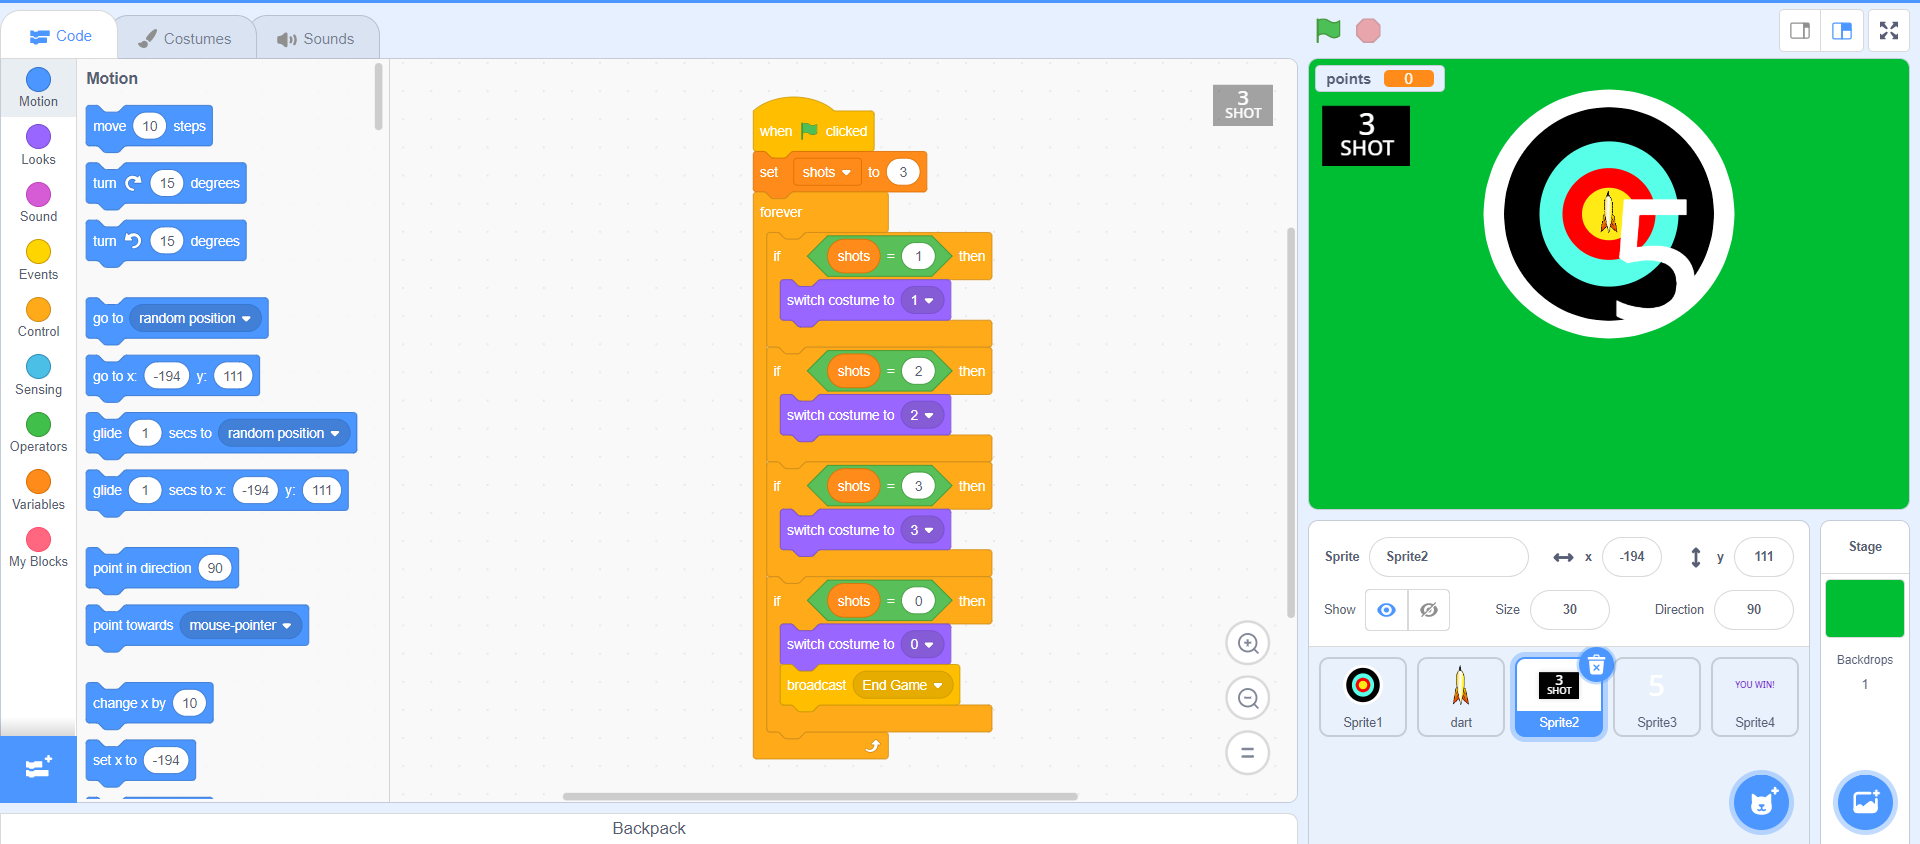
\includegraphics[width=1.0\linewidth,height=0.5\linewidth]{fig150014.png}
   \caption{Programming the number of shots}
\label{fig150014}
\end{figure}

\section{Programming the character that displays the number of points}

Select the character that shows how many points the player has earned. This hero, in addition to showing how many points there are, will also be responsible for reducing the number of shots, setting a new wind direction, as well as changing the status of the arrow to ready to shoot again.

Since you don't know how many points the player will earn, and to avoid doing thousands of checks, you can cross out the suit names by the number of points. So you can easily switch from suit to suit, since you have a variable that holds the number of points currently earned.

\begin{figure}[H]
   \centering
   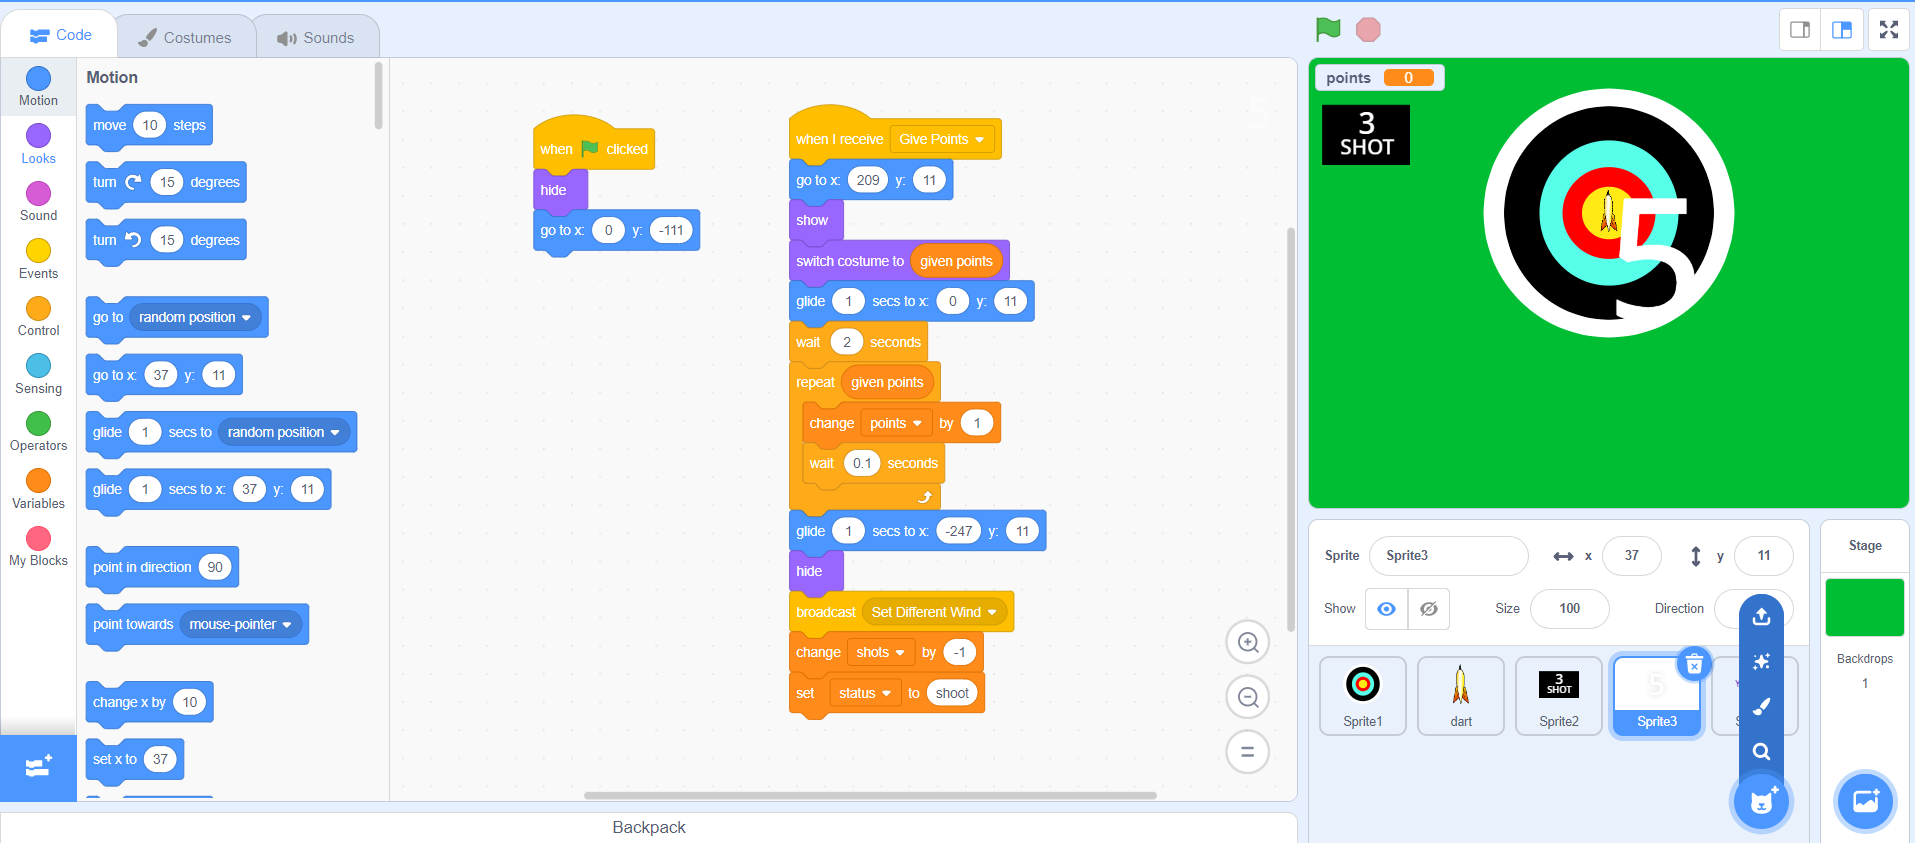
\includegraphics[width=1.0\linewidth,height=0.5\linewidth]{fig150015.png}
   \caption{Programming the number of points}
\label{fig150015}
\end{figure}

\section{Programming the end game}

The last step left to do is program the endgame. Depending on how many points the player has earned, he will either win or lose after the third shot. If the number of points is greater than 13 - he wins. Otherwise, he loses.

\begin{figure}[H]
   \centering
   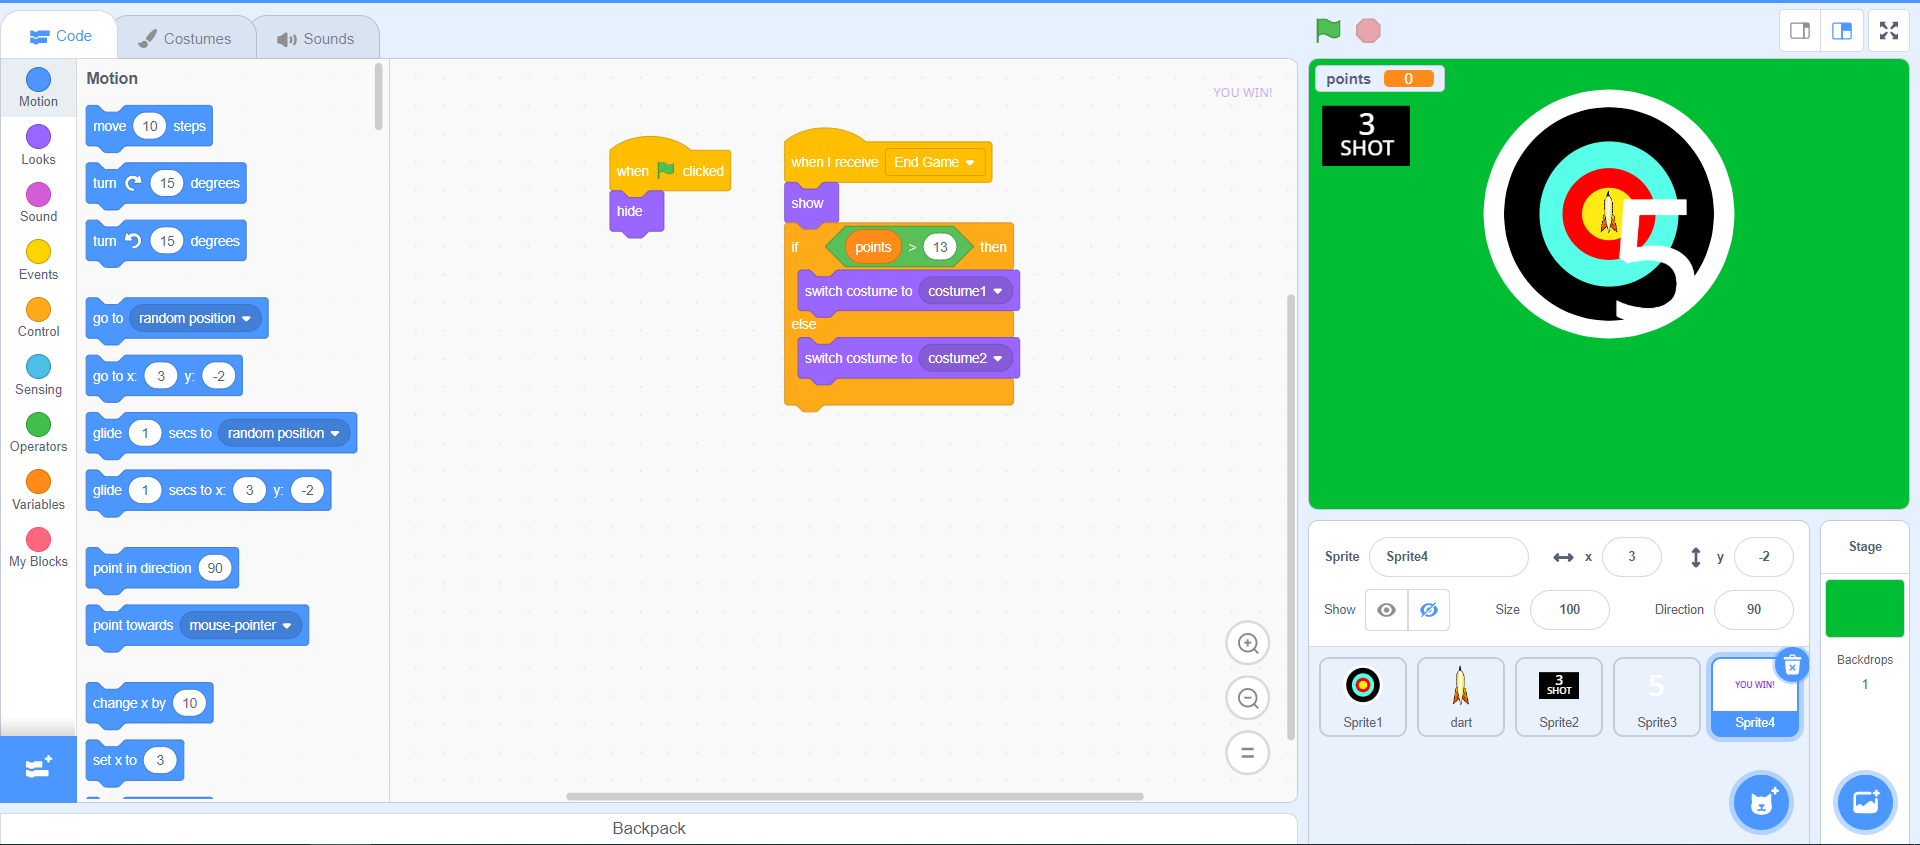
\includegraphics[width=1.0\linewidth,height=0.5\linewidth]{fig150016.png}
   \caption{Programming the end game}
\label{fig150016}
\end{figure}

You are ready to test how accurate and good you are in the game you created.
